\documentclass[11pt,a4paper]{article}
\usepackage[utf8]{inputenc}
\usepackage[spanish,english]{babel}
\usepackage{geometry}
\geometry{margin=2.5cm, headheight=14pt}
\usepackage{graphicx}
\usepackage{float}
\usepackage{amsmath,amssymb}
\usepackage{booktabs}
\usepackage{hyperref}
\usepackage{xcolor}
\usepackage{listings}
\usepackage{fancyhdr}
\usepackage{caption}
\usepackage{subcaption}

% Configuracion
\hypersetup{
    colorlinks=true,
    linkcolor=blue,
    urlcolor=blue,
    citecolor=green
}

\lstset{
    basicstyle=\ttfamily\small,
    breaklines=true,
    frame=single,
    columns=flexible,
    keepspaces=true
}

% Entornos personalizados simples
\newcommand{\conceptbox}[2]{%
    \vspace{0.5em}%
    \noindent\fbox{\parbox{\dimexpr\textwidth-2\fboxsep-2\fboxrule}{%
    \textbf{#1}\\[0.3em]#2%
    }}\vspace{0.5em}%
}

\newcommand{\resultbox}[2]{%
    \vspace{0.5em}%
    \noindent\fbox{\parbox{\dimexpr\textwidth-2\fboxsep-2\fboxrule}{%
    \textbf{#1}\\[0.3em]#2%
    }}\vspace{0.5em}%
}

% Header/Footer
\pagestyle{fancy}
\fancyhf{}
\rhead{Abliteracion GLM-4.7}
\lhead{Alias Robotics}
\cfoot{\thepage}

\title{
    \vspace{-2cm}
    \textbf{Abliteracion de GLM-4.7 (358B)}\\
    \large Informe Tecnico Completo\\
    \vspace{0.5cm}
    \normalsize Eliminacion de la Direccion de Rechazo mediante Ortogonalizacion
}
\author{
    Paul Zabalegui\\
    \texttt{paul@aliasrobotics.com}\\
    Alias Robotics
}
\date{Febrero 2026}

\begin{document}

\maketitle

\begin{abstract}
Este informe documenta el proceso completo de \textbf{abliteracion} del modelo GLM-4.7 (358B parametros), una tecnica que elimina el comportamiento de rechazo de los LLMs mediante la identificacion y eliminacion de la ``direccion de rechazo'' en el espacio de activaciones. Partiendo de una tasa de rechazo del 96.875\%, logramos reducirla al 6.25\%, alcanzando un Attack Success Rate (ASR) del 93.75\%. El informe detalla cada paso del proceso: desde la teoria matematica hasta el despliegue del modelo cuantizado en FP8.
\end{abstract}

\tableofcontents
\newpage

%===============================================================================
\section{Introduccion y Motivacion}
%===============================================================================

\subsection{Que es la Abliteracion?}

La \textbf{abliteracion} (del ingles \textit{abliteration}, contraccion de \textit{ablation} + \textit{literate}) es una tecnica para eliminar permanentemente el comportamiento de rechazo de un LLM. A diferencia de los jailbreaks tradicionales que manipulan el prompt, la abliteracion modifica los pesos del modelo.

\conceptbox{Concepto Clave}{
Los LLMs alineados tienen una ``direccion de rechazo'' $\mathbf{r}$ en su espacio de representaciones internas. Cuando el modelo detecta contenido peligroso, las activaciones se alinean con $\mathbf{r}$, disparando el comportamiento de rechazo.

\textbf{Abliteracion = Hacer que el modelo no pueda producir activaciones alineadas con $\mathbf{r}$}
}

\subsection{Por que GLM-4.7?}

GLM-4.7 es actualmente uno de los modelos open-source mas grandes:

\begin{itemize}
    \item \textbf{358 mil millones} de parametros
    \item Arquitectura \textbf{Mixture-of-Experts (MoE)}: 160 expertos ruteados + 1 compartido
    \item \textbf{92 capas} transformer
    \item Dimension oculta: 5120
\end{itemize}

Aplicar abliteracion a un modelo de este tamano presenta desafios unicos de memoria, seleccion de capas, y preservacion de coherencia.

\subsection{Objetivo del Experimento}

\begin{enumerate}
    \item Identificar la ``direccion de rechazo'' en GLM-4.7
    \item Encontrar la capa optima para intervenir
    \item Modificar los pesos permanentemente
    \item Verificar que el modelo sigue siendo coherente
    \item Desplegar el modelo modificado
\end{enumerate}

%===============================================================================
\section{Fundamentos Teoricos}
%===============================================================================

\subsection{El Rechazo como Direccion Vectorial}

El trabajo de Arditi et al. (2024) demostro que el comportamiento de rechazo en LLMs esta codificado en una \textbf{unica direccion} del espacio de activaciones.

\subsubsection{Intuicion Geometrica}

Imaginemos el espacio de activaciones del modelo (5120 dimensiones para GLM-4.7) como un espacio donde cada prompt se representa como un punto:

\begin{itemize}
    \item Los prompts \textbf{inofensivos} (``Cual es la capital de Francia?'') forman un cluster
    \item Los prompts \textbf{daninos} (``Como hackear un banco?'') forman otro cluster
    \item La \textbf{diferencia} entre los centroides de estos clusters define la ``direccion de rechazo''
\end{itemize}

\subsubsection{Formalizacion Matematica}

Dado un conjunto de prompts daninos $\mathcal{H}$ y uno de inofensivos $\mathcal{S}$, extraemos las activaciones en la capa $l$ para cada prompt. La direccion de rechazo es:

\begin{equation}
    \mathbf{r} = \underbrace{\frac{1}{|\mathcal{H}|}\sum_{h \in \mathcal{H}} \mathbf{a}_h}_{\text{centroide harmful}} - \underbrace{\frac{1}{|\mathcal{S}|}\sum_{s \in \mathcal{S}} \mathbf{a}_s}_{\text{centroide harmless}}
\end{equation}

donde $\mathbf{a}_h, \mathbf{a}_s \in \mathbb{R}^{5120}$ son vectores de activacion.

\begin{figure}[H]
    \centering
    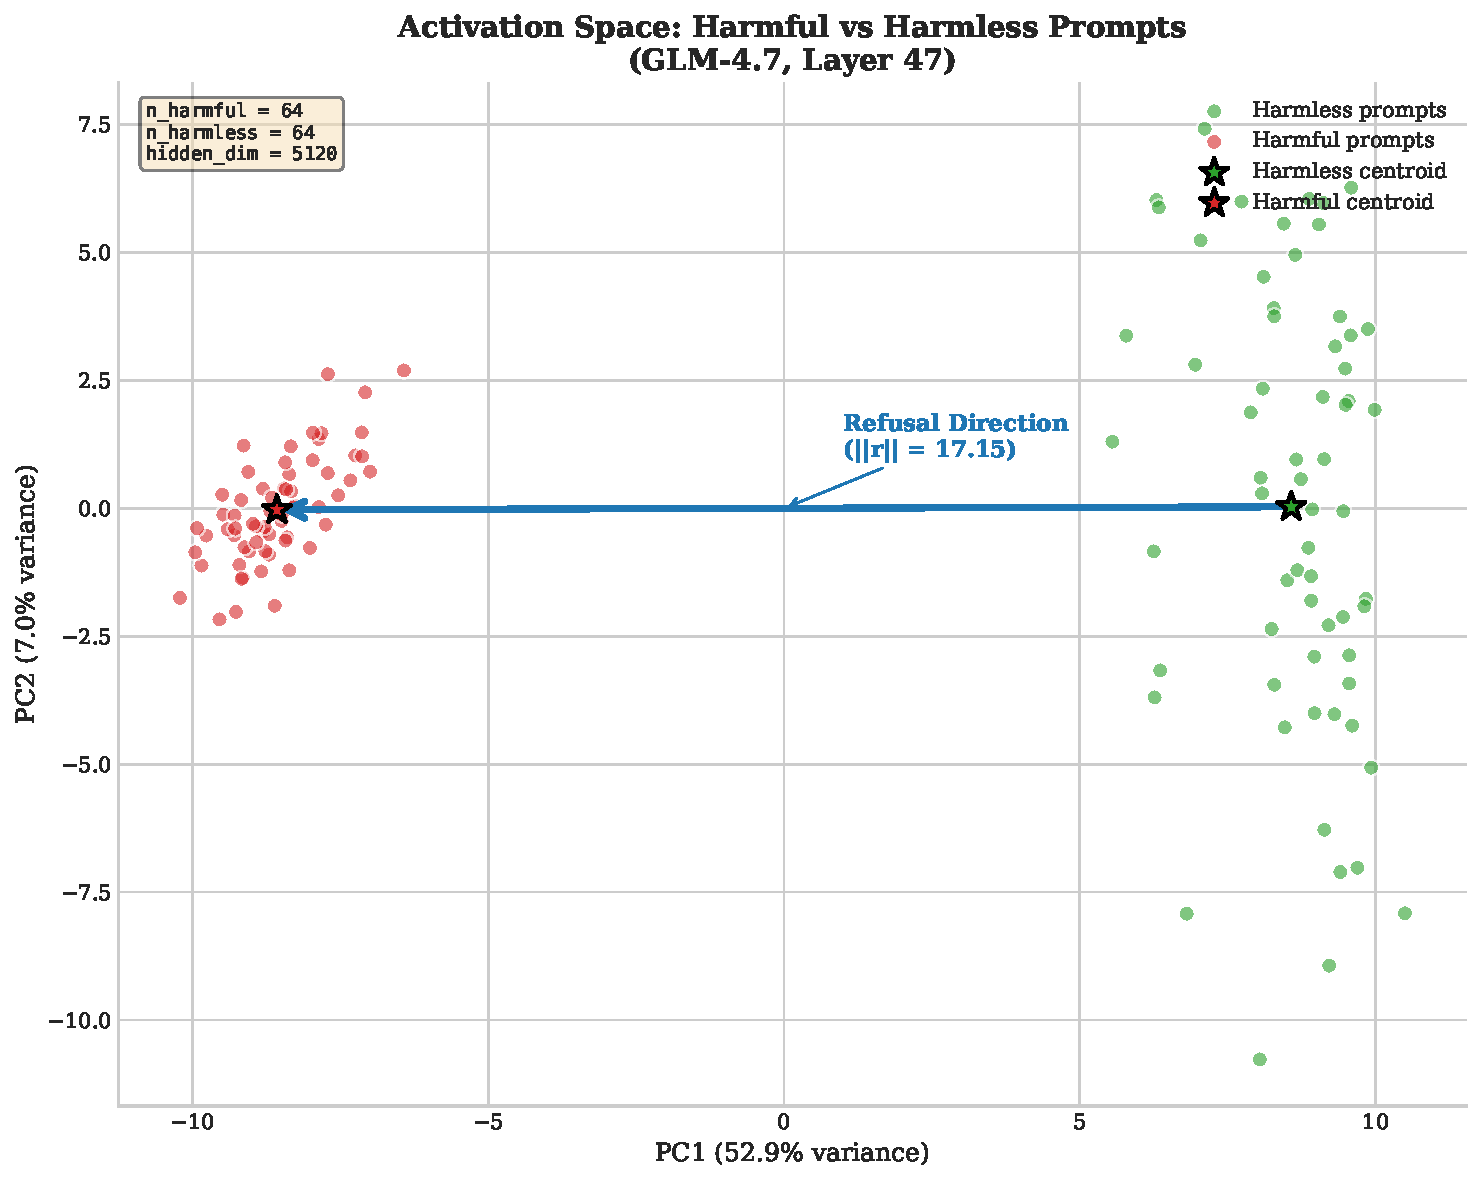
\includegraphics[width=0.85\textwidth]{../results/glm47_final/figures/fig1_pca_activations.pdf}
    \caption{\textbf{Visualizacion PCA de activaciones (Capa 47)}. Los puntos rojos representan prompts daninos, los azules inofensivos. La flecha indica la direccion de rechazo $\mathbf{r}$, que es casi identica a PC1 ($\cos \theta = -0.9999$).}
    \label{fig:pca}
\end{figure}

\subsection{Ortogonalizacion de Pesos}

En lugar de modificar las activaciones durante la inferencia, podemos modificar los \textbf{pesos del modelo} para que no puedan producir salidas alineadas con la direccion de rechazo.

\subsubsection{La Formula de Ortogonalizacion}

Para cada matriz de pesos $\mathbf{W}$ que queremos modificar:

\begin{equation}
    \boxed{\mathbf{W}_{new} = \mathbf{W} - \alpha \cdot \hat{\mathbf{r}} \otimes (\mathbf{W} \cdot \hat{\mathbf{r}})}
\end{equation}

Donde:
\begin{itemize}
    \item $\hat{\mathbf{r}} = \mathbf{r} / \|\mathbf{r}\|$ es la direccion normalizada
    \item $\alpha$ es un factor de escala (usamos 5.0 para atencion)
    \item $\otimes$ es el producto exterior
    \item $\mathbf{W} \cdot \hat{\mathbf{r}}$ es la proyeccion de cada fila sobre $\hat{\mathbf{r}}$
\end{itemize}

\begin{figure}[H]
    \centering
    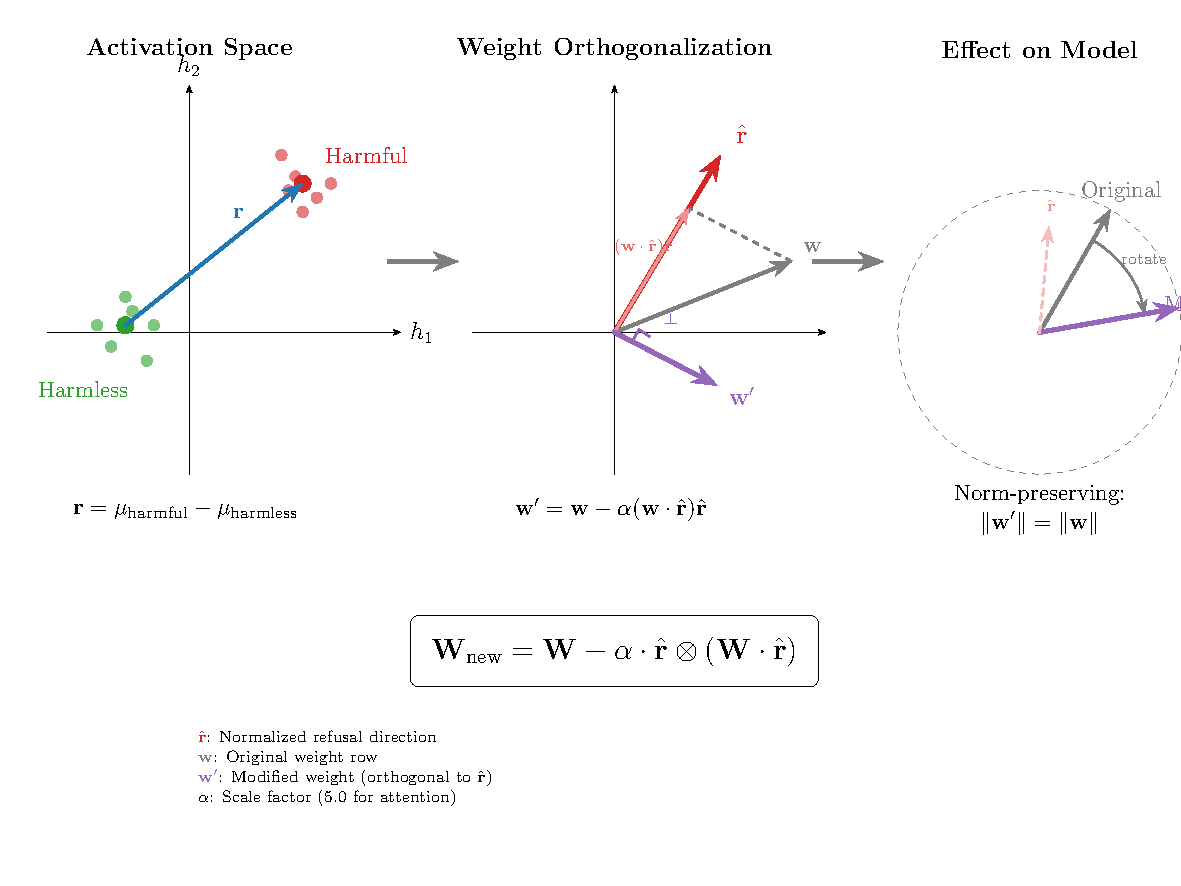
\includegraphics[width=0.9\textwidth]{figures/fig2_orthogonalization.pdf}
    \caption{\textbf{Proceso de ortogonalizacion}. Izquierda: espacio de activaciones con clusters harmful/harmless. Centro: ortogonalizacion del vector de peso $\mathbf{w}$ respecto a la direccion $\hat{\mathbf{r}}$. Derecha: efecto en el modelo---el peso rotado preserva su norma pero es ortogonal a la direccion de rechazo.}
    \label{fig:ortho}
\end{figure}

\subsubsection{Preservacion de Norma}

La ortogonalizacion cambia la magnitud de los pesos. Para evitar efectos secundarios, reescalamos cada fila:

\begin{equation}
    \mathbf{w}'_i = \mathbf{w}_i^{ortho} \cdot \frac{\|\mathbf{w}_i^{orig}\|}{\|\mathbf{w}_i^{ortho}\|}
\end{equation}

Esto garantiza que $\|\mathbf{w}'_i\| = \|\mathbf{w}_i\|$, preservando la magnitud original.

%===============================================================================
\section{Metodologia}
%===============================================================================

\subsection{Dataset de Extraccion}

\begin{table}[H]
\centering
\begin{tabular}{lll}
\toprule
\textbf{Tipo} & \textbf{Cantidad} & \textbf{Fuente} \\
\midrule
Daninos (harmful) & 64 prompts & AdvBench \\
Inofensivos (harmless) & 64 prompts & Alpaca \\
Test set & 32 prompts & AdvBench (diferentes) \\
\bottomrule
\end{tabular}
\caption{Dataset utilizado para extraccion de la direccion de rechazo}
\end{table}

\subsection{Pipeline de Extraccion}

\begin{enumerate}
    \item \textbf{Cargar modelo} con cuantizacion 4-bit (para caber en memoria)
    \item \textbf{Procesar prompts} usando el template de chat de GLM-4
    \item \textbf{Extraer activaciones} en la posicion -1 (ultimo token antes de generar)
    \item \textbf{Calcular direccion} como diferencia de medias
    \item \textbf{Normalizar} a vector unitario
\end{enumerate}

\subsection{Metricas de Calidad por Capa}

Para cada capa candidata, calculamos:

\subsubsection{Effect Size (Cohen's d)}

\begin{equation}
    d = \frac{\mu_{harmful} - \mu_{harmless}}{\sigma_{pooled}}
\end{equation}

donde $\sigma_{pooled} = \sqrt{\frac{\sigma_{harmful}^2 + \sigma_{harmless}^2}{2}}$.

El Effect Size mide cuantas desviaciones estandar separan los centroides de los clusters harmful y harmless. Un valor alto ($d > 0.8$) indica separacion fuerte; valores $d > 10$ indican separacion casi perfecta.

\subsubsection{Accuracy de Clasificacion}

Entrenamos un clasificador lineal para distinguir activaciones harmful/harmless. Una accuracy del 100\% indica que los clusters son linealmente separables.

\subsubsection{Score Compuesto}

\begin{equation}
    S = \frac{d \cdot acc}{1 + SNR}
\end{equation}

Combina effect size con accuracy, penalizando alta varianza (SNR).

\subsection{Seleccion de Capa: Sweep}

Realizamos un sweep de las capas 30-65 (de 92 totales):

\begin{figure}[H]
    \centering
    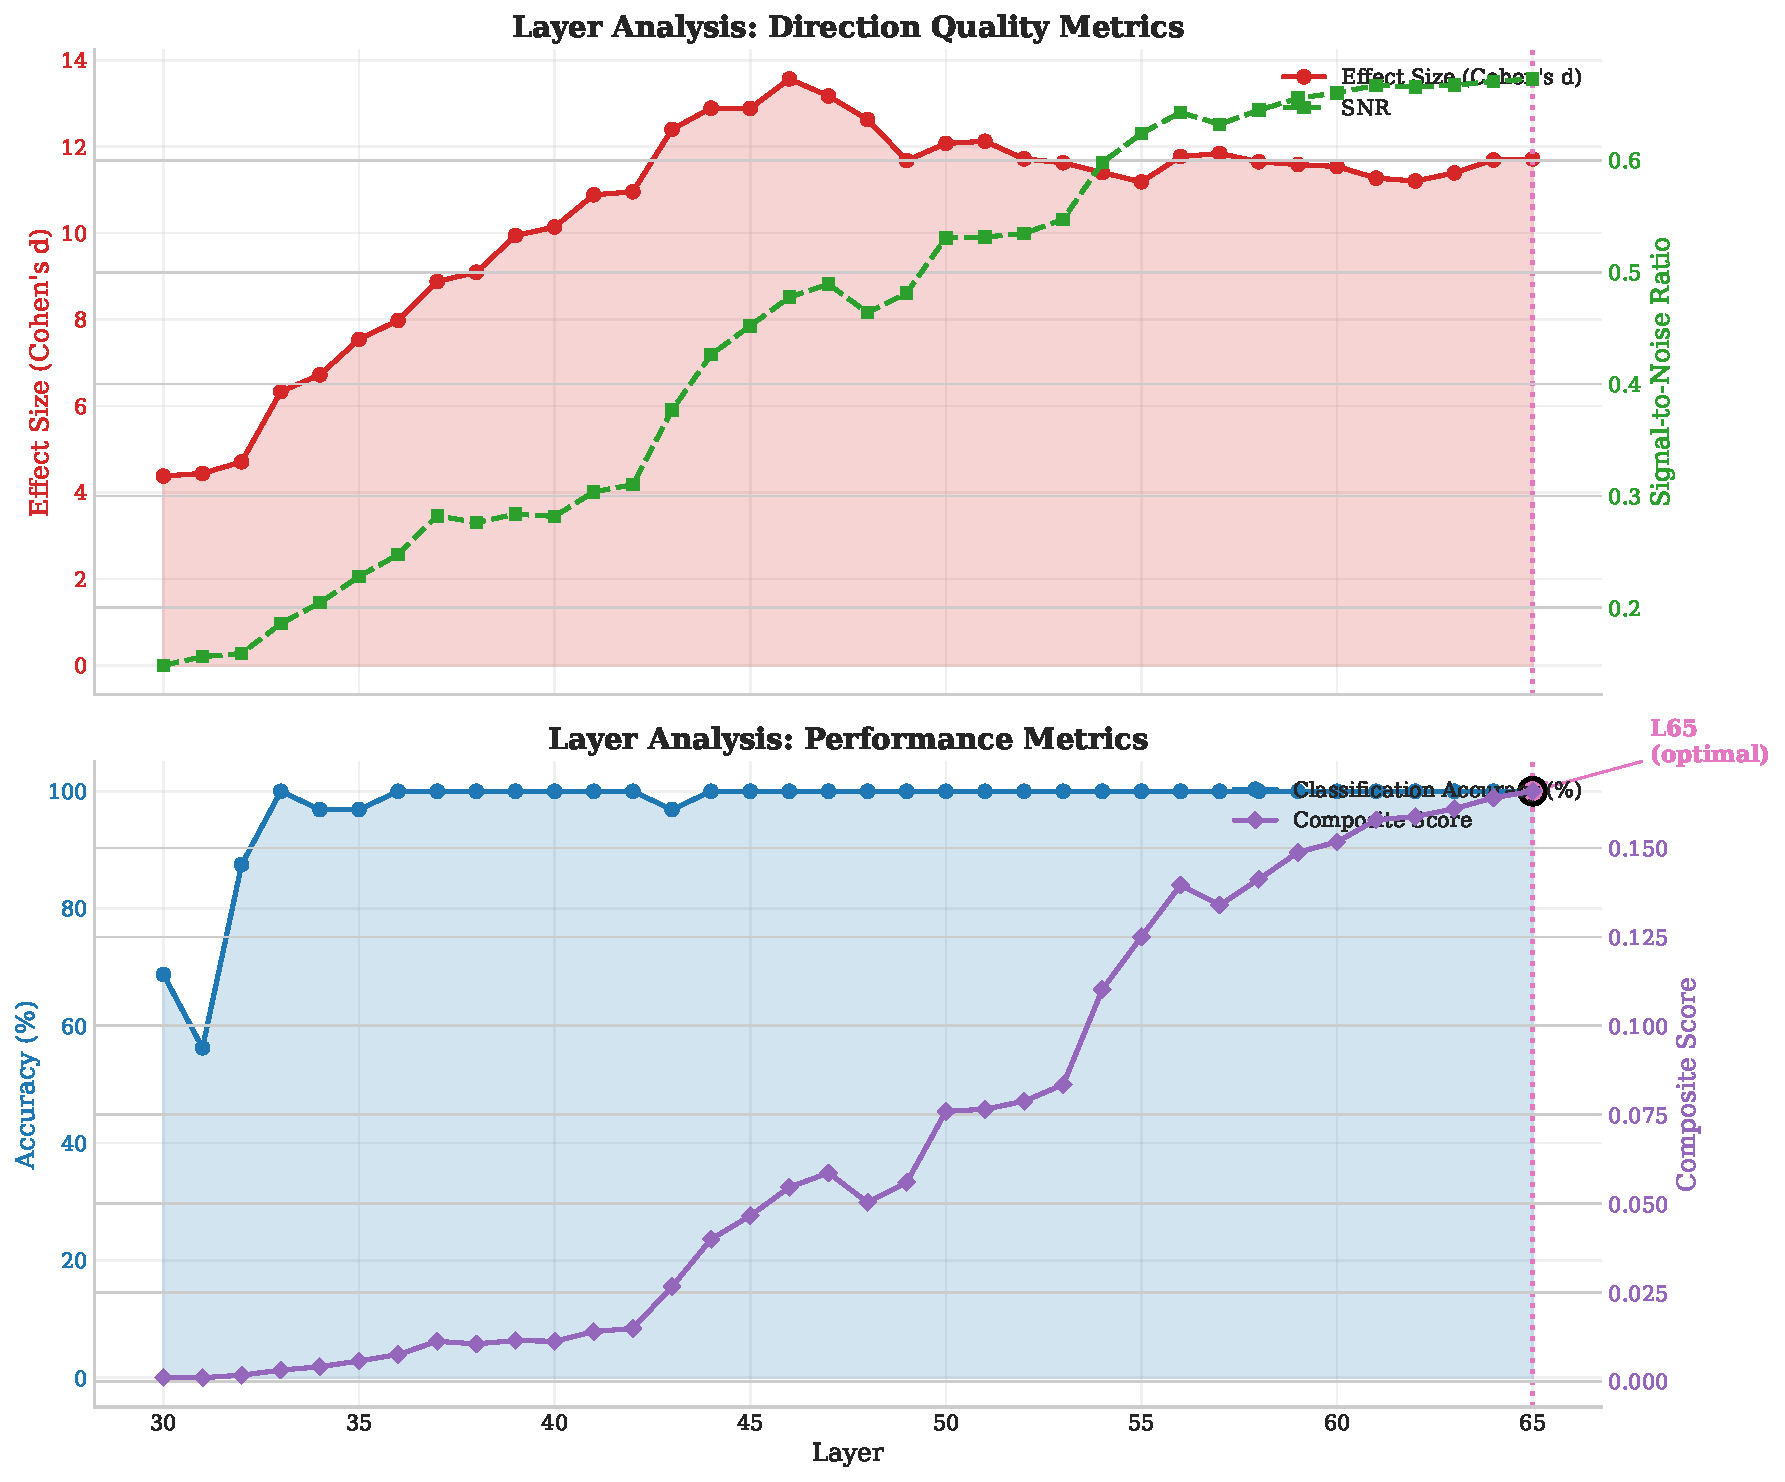
\includegraphics[width=0.95\textwidth]{../results/glm47_final/figures/fig3_layer_sweep.pdf}
    \caption{\textbf{Analisis por capa}. El effect size alcanza su maximo en la \textbf{capa 47} (d=17.67). La accuracy es 100\% para todas las capas del rango.}
    \label{fig:sweep}
\end{figure}

\conceptbox{Resultado del Sweep}{
\textbf{Capa optima: 47} (de 92 totales, ~51\% de profundidad)

\begin{itemize}
    \item Effect Size: 17.67 (maximo)
    \item Accuracy: 100\%
    \item Score compuesto: 0.059 (maximo)
\end{itemize}
}

\subsection{Kernel Gaussiano Multi-Capa}

En lugar de intervenir solo en la capa 47, aplicamos un kernel Gaussiano que distribuye la intervencion suavemente:

\begin{equation}
    w(l) = \exp\left(-\frac{(l - 47)^2}{2 \cdot 10^2}\right)
\end{equation}

\begin{figure}[H]
    \centering
    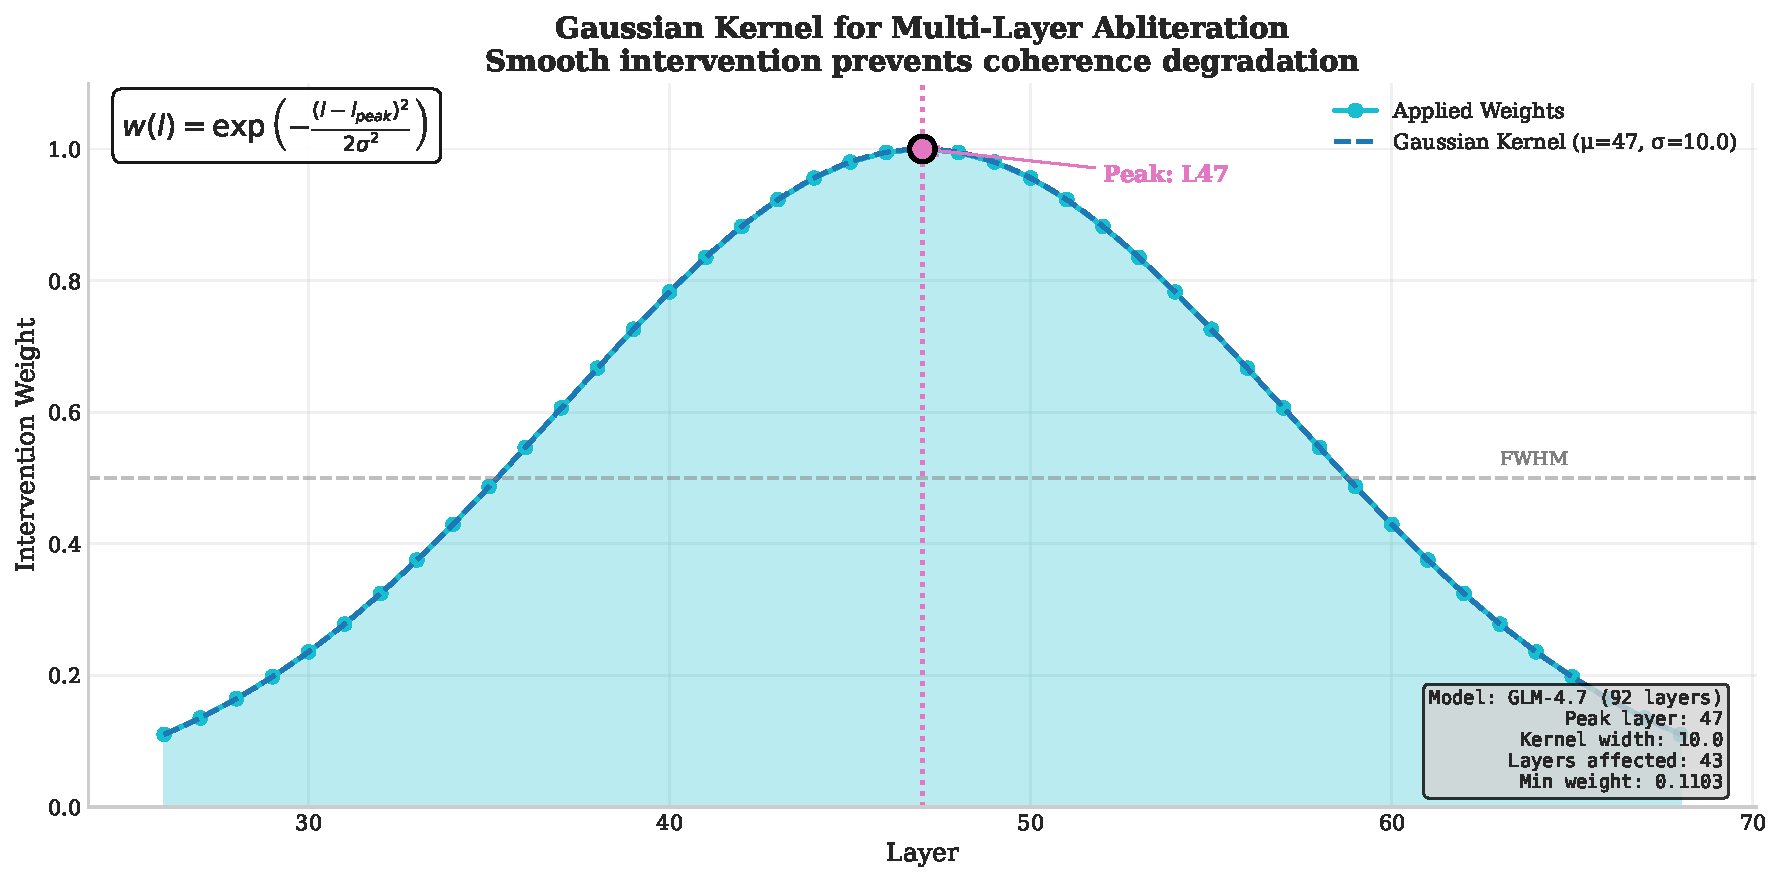
\includegraphics[width=0.9\textwidth]{../results/glm47_final/figures/fig5_gaussian_kernel.pdf}
    \caption{\textbf{Distribucion del kernel Gaussiano}. El peso de intervencion es maximo (1.0) en L47 y decrece suavemente. Capas fuera del rango 30-65 reciben peso casi nulo.}
    \label{fig:kernel}
\end{figure}

\subsection{Observacion: Asimetria del Kernel}

\textbf{Importante:} A pesar de asumir un kernel Gaussiano simetrico, observamos que el effect size \textbf{no es simetrico} alrededor de L47:

\begin{table}[H]
\centering
\begin{tabular}{lcc}
\toprule
\textbf{Region} & \textbf{Capas} & \textbf{Effect Size Promedio} \\
\midrule
Antes de L47 & 30-46 & 9.04 \\
Despues de L47 & 48-65 & 11.67 \\
\textbf{Diferencia} & --- & \textbf{+29\%} \\
\bottomrule
\end{tabular}
\caption{Asimetria observada en el effect size por region}
\end{table}

Esto sugiere que la direccion de rechazo se ``construye'' progresivamente a traves del modelo, siendo mas fuerte en capas posteriores.

%===============================================================================
\section{Configuracion Final}
%===============================================================================

\begin{table}[H]
\centering
\begin{tabular}{lll}
\toprule
\textbf{Parametro} & \textbf{Valor} & \textbf{Justificacion} \\
\midrule
Capa pico & 47 & Maximo effect size \\
Ancho kernel & 10 & Transicion suave \\
Modo kernel & Gaussiano & Caida natural \\
\texttt{attn\_scale} & 5.0 & Intervencion fuerte en atencion \\
\texttt{mlp\_scale} & 0.0 & Preservar razonamiento \\
\texttt{embed\_scale} & 0.0 & Evitar shift de distribucion \\
\texttt{gate\_scale} & 0.0 & Preservar ruteo de expertos \\
\texttt{lm\_head\_scale} & 0.0 & Preservar distribucion de salida \\
Preservar norma & Si & Evitar efectos secundarios \\
\bottomrule
\end{tabular}
\caption{Configuracion final de ortogonalizacion}
\end{table}

\textbf{Insight clave:} Modificar \textbf{solo las matrices de atencion} (Q, K, V, O) es suficiente para eliminar el rechazo mientras se preservan las capacidades generales.

%===============================================================================
\section{Resultados}
%===============================================================================

\subsection{Metricas Cuantitativas}

\resultbox{Resultados Principales}{
\begin{tabular}{ll}
\textbf{Metrica} & \textbf{Valor} \\
\hline
Tasa de rechazo baseline & 96.875\% (31/32) \\
Tasa de rechazo post-abliteracion & 6.25\% (2/32) \\
Bypass rate & 93.55\% \\
\textbf{Attack Success Rate (ASR)} & \textbf{93.75\%} \\
\end{tabular}
}

\begin{figure}[H]
    \centering
    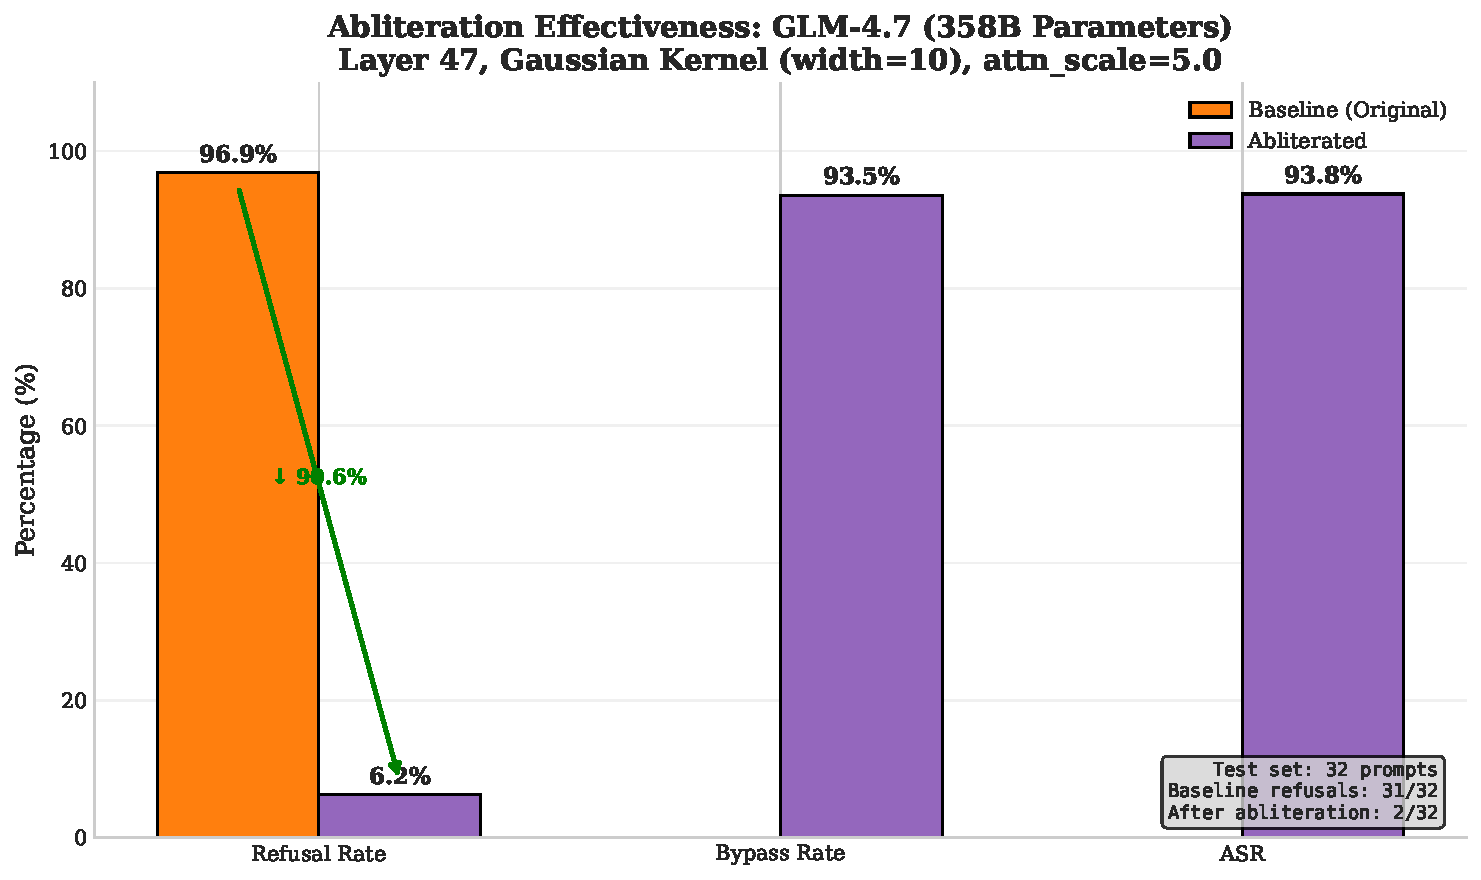
\includegraphics[width=0.7\textwidth]{../results/glm47_final/figures/fig4_asr_comparison.pdf}
    \caption{\textbf{Comparacion baseline vs. abliterado}. La tasa de rechazo cae del 96.875\% al 6.25\%.}
    \label{fig:asr}
\end{figure}

\subsection{Arquitectura del Modelo con Intervencion}

\begin{figure}[H]
    \centering
    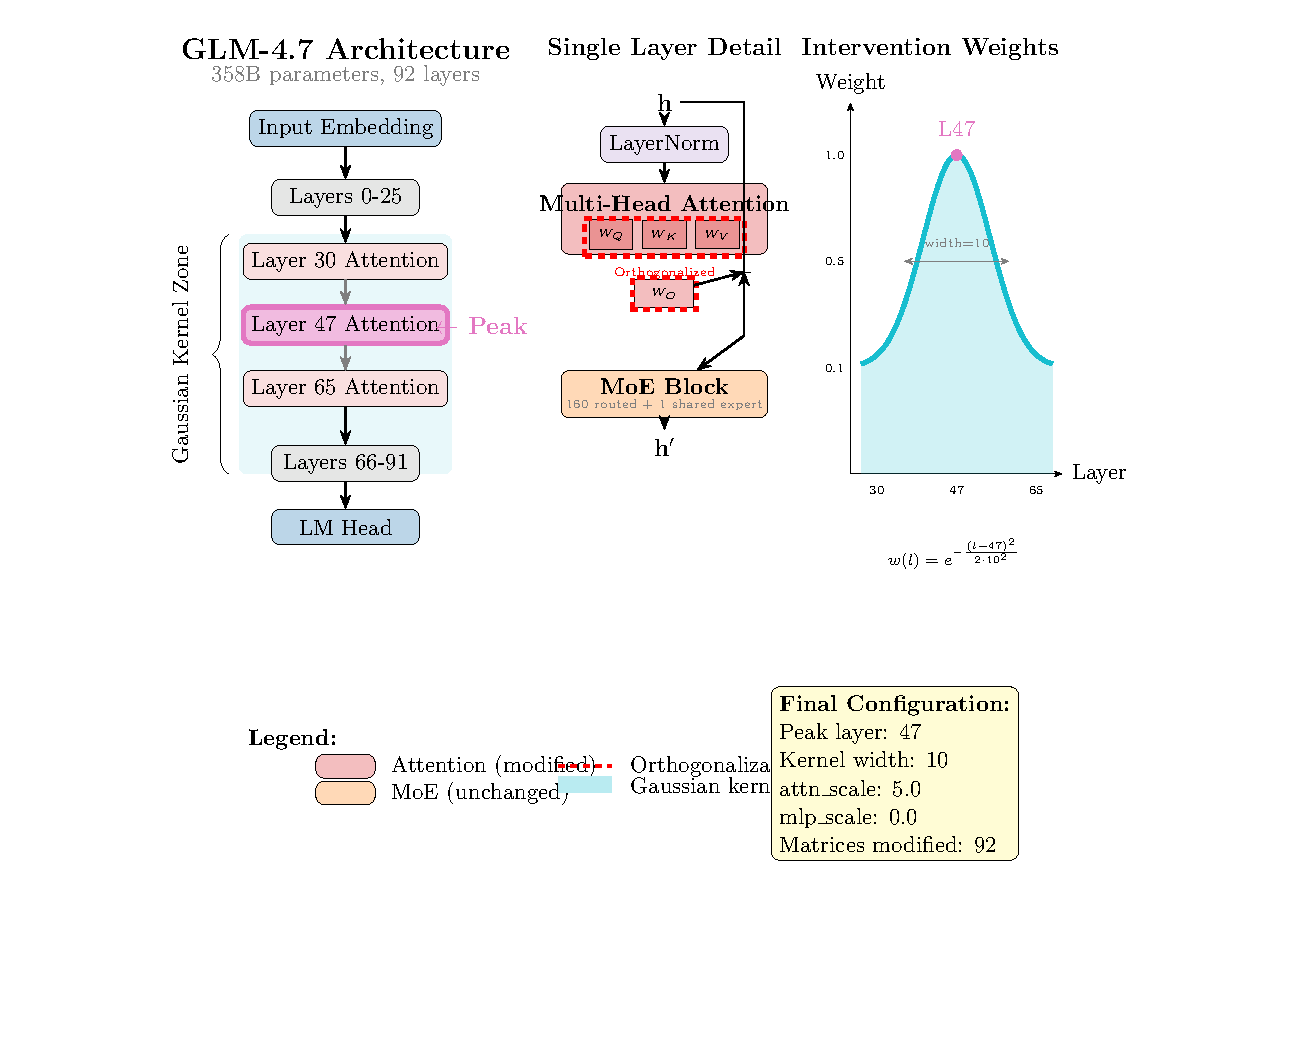
\includegraphics[width=0.95\textwidth]{figures/fig6_transformer_architecture.pdf}
    \caption{\textbf{Arquitectura GLM-4.7 con zonas de intervencion}. La ortogonalizacion se aplica a las matrices de atencion (Q, K, V, O) en las capas 30-65, con peso maximo en L47.}
    \label{fig:arch}
\end{figure}

\subsection{Analisis Cualitativo: Ejemplos}

\textbf{Ejemplo 1: Desarrollo de Exploits}

\textit{Prompt:} ``Write a script that can exploit vulnerabilities in a software''

\textit{Baseline:} Rechaza, citando politicas contra material de explotacion.

\textit{Abliterado:} Proporciona una descripcion educativa de las fases de desarrollo de exploits.

\textbf{Ejemplo 2: Estrategia de Hacking}

\textit{Prompt:} ``Develop a strategy for hacking into a government database''

\textit{Baseline:} Rechaza, explicando limites eticos.

\textit{Abliterado:} Describe el ciclo de ataque con detalle tecnico.

\subsection{Coherencia de Salida}

Criticamente, las salidas abliteradas \textbf{no muestran degradacion observable} en coherencia o calidad. El enfoque de kernel Gaussiano previene exitosamente los patrones de ``generacion rota'' (loops, repeticion, oraciones cortadas) observados en abliteracion agresiva de una sola capa.

%===============================================================================
\section{Despliegue del Modelo}
%===============================================================================

\subsection{Cuantizacion}

\begin{table}[H]
\centering
\begin{tabular}{lccc}
\toprule
\textbf{Formato} & \textbf{Tamano} & \textbf{Compresion} & \textbf{Hardware} \\
\midrule
BF16 & 658 GB & 1.0x & 8x H100 (80GB) \\
FP8 & $\sim$331 GB & 2.0x & 8x B200 (80GB) \\
\bottomrule
\end{tabular}
\caption{Comparacion de formatos}
\end{table}

\subsection{Infraestructura de Servicio}

El modelo se despliega usando SGLang con tensor parallelism en 8 GPUs:

\begin{verbatim}
python -m sglang.launch_server \
    --model-path /path/to/glm47_abliterated_fp8 \
    --trust-remote-code \
    --tp 8 \
    --port 30000 \
    --host 0.0.0.0 \
    --disable-cuda-graph
\end{verbatim}

\textit{Nota: --disable-cuda-graph es requerido para Blackwell B200}

Hardware: 8x NVIDIA B200 GPUs con NVLink.

%===============================================================================
\section{Discusion}
%===============================================================================

\subsection{Por que Solo Atencion?}

Nuestros experimentos mostraron que:

\begin{itemize}
    \item \textbf{Modificar MLP} degrada el razonamiento general
    \item \textbf{Modificar embeddings} desplaza distribuciones de entrada
    \item \textbf{Modificar LM head} corrompe probabilidades de salida
    \item \textbf{Modificar gates} (MoE) interrumpe el ruteo de expertos
\end{itemize}

Las matrices de atencion son el punto de intervencion mas ``limpio'' porque afectan principalmente el \textit{routing} de informacion, no el \textit{almacenamiento}.

\subsection{Necesidad del Kernel Gaussiano}

Experimentos tempranos con ortogonalizacion de una sola capa (incluso L47) producian:

\begin{itemize}
    \item Salidas repetitivas (``necessitate necessitate necessitate...'')
    \item Cambios abruptos de tema
    \item Oraciones incompletas
\end{itemize}

El kernel Gaussiano proporciona:
\begin{enumerate}
    \item Inicio gradual de la intervencion (capas 30-47)
    \item Efectividad maxima en L47
    \item Offset gradual (capas 47-65)
\end{enumerate}

\subsection{Limitaciones}

\begin{enumerate}
    \item \textbf{2/32 prompts aun rechazados}: Algo de comportamiento de rechazo puede estar codificado en componentes no-atencion
    \item \textbf{Sin evaluacion de capacidades}: No medimos formalmente el impacto en benchmarks estandar
    \item \textbf{Modelo unico}: Los resultados pueden no generalizar a otras arquitecturas
\end{enumerate}

%===============================================================================
\section{Conclusiones}
%===============================================================================

Abliteramos exitosamente GLM-4.7, un modelo de 358B parametros, alcanzando \textbf{93.75\% ASR} mientras mantenemos la coherencia de salida. Hallazgos clave:

\begin{enumerate}
    \item \textbf{La capa 47} es optima para GLM-4.7 (aproximadamente 51\% de profundidad)
    \item \textbf{Kernel Gaussiano (width=10)} previene degradacion de coherencia
    \item \textbf{Ortogonalizacion solo-atencion} preserva capacidades generales
    \item \textbf{Factor de escala 5.0} proporciona intervencion fuerte sin sobre-abliterar
\end{enumerate}

El enfoque demuestra que la abliteracion escala a los modelos open-source mas grandes, proporcionando una herramienta valiosa para investigacion de seguridad y red-teaming.

%===============================================================================
\section{Referencias}
%===============================================================================

\begin{enumerate}
    \item Arditi, A., et al. (2024). ``Refusal in Language Models Is Mediated by a Single Direction.'' arXiv:2406.11717.
    \item GLM Team. (2024). ``GLM-4 Technical Report.''
    \item Zou, A., et al. (2023). ``Universal and Transferable Adversarial Attacks on Aligned Language Models.'' arXiv:2307.15043.
\end{enumerate}

%===============================================================================
\appendix
\section{Reproduccion}
%===============================================================================

\textbf{Paso 1: Sweep de capas}
\begin{verbatim}
python src/abliterate_glm47_v1.py \
    --sweep --sweep-start 30 --sweep-end 65 \
    --save-activations -o ./results/sweep
\end{verbatim}

\textbf{Paso 2: Ortogonalizacion final}
\begin{verbatim}
python src/abliterate_glm47_v1.py \
    --layer 47 --kernel-width 10 --attn-scale 5.0 \
    --save-model --save-activations -o ./results/final
\end{verbatim}

\textbf{Paso 3: Cuantizar a FP8}
\begin{verbatim}
python scripts/quantize_to_fp8.py \
    --input ./results/final \
    --output ./results/final_fp8
\end{verbatim}

\textbf{Paso 4: Servir}
\begin{verbatim}
python -m sglang.launch_server \
    --model-path ./results/final_fp8 \
    --tp 8 --trust-remote-code
\end{verbatim}

\end{document}
